\documentclass{article}
\usepackage{tikz}
\usetikzlibrary{arrows.meta}

\begin{document}

\begin{center}
    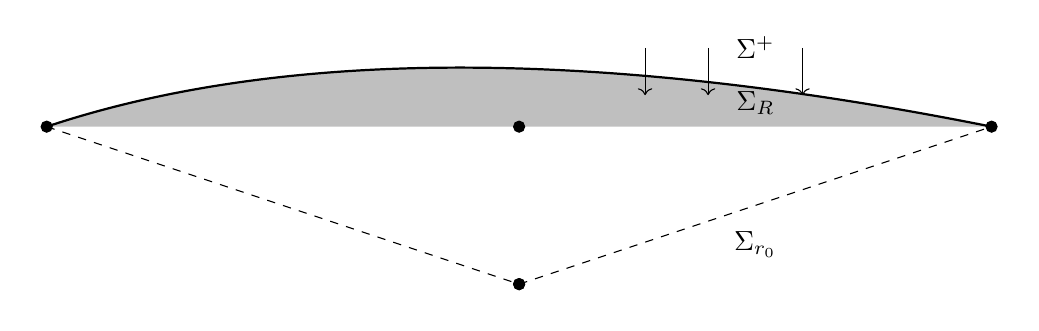
\begin{tikzpicture}[scale=2]
        % Define coordinates
        \coordinate (A) at (-3, 0);
        \coordinate (B) at (0, -1); 
        \coordinate (C) at (3, 0);
        \coordinate (D) at (0, 0);

        % Draw the boundary line
        \draw[dashed] (A) -- (B) -- (C);
        
        % Draw the inner curve
        \draw[thick, fill=gray!50] (A) .. controls (-1.5, 0.5) and (0.5, 0.5) .. (C);
        
        % Add labels for the hypersurfaces
        \node at (1.5, 0.5) {$\Sigma^+$};
        \node at (1.5, 0.15) {$\Sigma_R$};
        \node at (1.5, -0.75) {$\Sigma_{r_0}$};

        % Draw the vertical lines
        \draw[->] (1.2, 0.5) -- (1.2, 0.2);
        \draw[->] (0.8, 0.5) -- (0.8, 0.2);
        \draw[->] (1.8, 0.5) -- (1.8, 0.2);
        
        % Mark the endpoints and the central point
        \filldraw (A) circle (1pt) node[left] {};
        \filldraw (B) circle (1pt) node[below] {};
        \filldraw (C) circle (1pt) node[right] {};
        \filldraw (D) circle (1pt) node[above] {};
        
        % Draw the central point
        \filldraw (0, -1) circle (1pt);
    \end{tikzpicture}
\end{center}

\textbf{Description:} The figure illustrates the spacetime region used to solve the wave equation within the expanding region. A sequence of finite problems is considered, starting from a solution $\psi_R$ defined on $\Sigma_R$ with prescribed data, and then showing that the limit $\lim_{R \to \infty} \psi_R$ exists in an appropriate energy space. This process is carried out up to a $\Sigma_{r_0}$ hypersurface, where $r_0 > r_{\mathcal{C}}$.

\end{document}